\documentclass[12pt]{article}

% --- Packages ---
\usepackage[utf8]{inputenc}      % character encoding
\usepackage[T1]{fontenc}         % better font encoding
\usepackage{lmodern}             % Latin Modern font
\usepackage{geometry}            % adjust page margins
\usepackage{setspace}            % line spacing
\usepackage{graphicx}            % insert images
\usepackage{amsmath, amssymb}    % math symbols
\usepackage{enumitem}            % better control of lists
\usepackage{hyperref}            % clickable links in PDF
\usepackage{xurl}                % enables better URL breaks
\usepackage{microtype}           % nicer line breaking/kerning
\usepackage[style=apa]{biblatex} % references
\usepackage{tikz}                % for cute diagram
\usepackage{pgfplots}            % for creating plots


% --- Page Setup ---
\geometry{margin=1in}
\setstretch{1.2}                 % slightly more spacing for readability
\addbibresource{references.bib}  % point to .bib file
\usetikzlibrary{arrows.meta,positioning,shapes.geometric,trees}
\usepgfplotslibrary{statistics} % boxplots from data
\pgfplotsset{compat=1.18}       % or your installed version



% --- Relative Frequency Table Formatting ---
% Command for tally group of up to 5
\newcommand{\tally}[1]{%
  \begin{tikzpicture}[scale=0.15,baseline=-0.5ex]
    \foreach \i in {1,...,#1} {
      \ifnum\i<5
        \draw (\i,0) -- (\i,1.5);
      \fi
      \ifnum\i=5
        \draw (1,0) -- (5,1.5);
      \fi
    }
  \end{tikzpicture}%
}


% --- Document Info ---
\title{\textbf{Probability \& Statistics}}
\author{Giorgina Gottlieb}
\date{Fall 2025}

\begin{document}

\maketitle

% ------------------ Vocabulary --------------------------------------
\section{Vocabulary}

\subsection{Data Sets}
    \begin{itemize}
        \item Population ($\mathcal{P}$): well-defined data set, and by well-defined, we mean the parameters are clear and specific
            \begin{itemize}[label=--]
            \item Concrete: all objects or individuals currently exist
            \item Conceptual/hypothetical: some or all objects or individuals do not exist or do not yet exist
            \end{itemize}
        \item Census: when the desired information is available for all objects in a population
        \item Sample: a subset of the population
            \begin{itemize}[label=--]
                \item Simple random sample: any particular subset of a specified size where objects or individuals have the same chance of being selected
                \item Stratified sample: where the population units are separated into nonoverlapping groups and a sample is taken from each
                \item Convenience sample: individuals or objects are selected without systematic randomization
            \end{itemize}
        \item[] \textit{Note: A sample of at least 30 is often considered to be sufficient (sometimes less)}
    \end{itemize}

\subsection{Branches of Statistics}
    \begin{itemize}
        \item Descriptive: summarize and visualize data observed (e.g., graphs, mean, median, etc.)
        \item Inferential: use sample data and probability to make claims about a population
        \item[] \textit{Note: Inference would not be necessary if we had the entire population} 
    \end{itemize}

% --- Relational Visual ---
\begin{center}
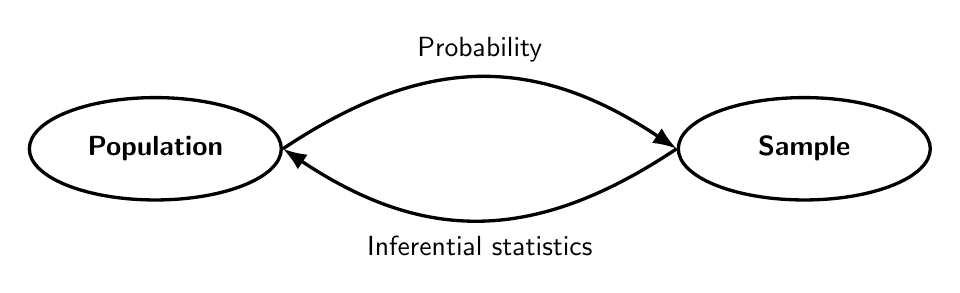
\begin{tikzpicture}[>=Latex, every node/.style={font=\sffamily}]
  % Nodes
  \node[draw, ellipse, very thick, minimum width=32mm, minimum height=13mm]
        (pop) {\textbf{Population}};
  \node[draw, ellipse, very thick, minimum width=32mm, minimum height=13mm,
        right=50mm of pop]
        (samp) {\textbf{Sample}};

  % Curved arrows with labels
  \draw[-{Latex[length=3mm]}, very thick]
    (pop.east) .. controls +(18mm,12mm) and +(-18mm,12mm) ..
    (samp.west)
      node[midway, above, yshift=2pt] {Probability};

  \draw[-{Latex[length=3mm]}, very thick]
    (samp.west) .. controls +(-18mm,-12mm) and +(18mm,-12mm) ..
    (pop.east)
      node[midway, below, yshift=-2pt] {Inferential statistics};
\end{tikzpicture}
\end{center}
% --- Relational Visual ---

\subsection{Data Type}
    \begin{itemize}
        \item Qualitative: categorical; non-numerical data or a number with \textbf{no numerical ordering} (e.g., a zip code)
        \item Quantitative: numerically ordered data
        \begin{itemize}[label=--]
            \item Discrete: where it is practical to list \textbf{all possible values} (e.g., counts)
            \item Continuous: where it is \textbf{not} practical to list all possible values (e.g., weights)
        \end{itemize}
    \end{itemize}

\subsection{Variables}
    \begin{itemize}
        \item Variable: any characteristic whose value may change from one object to another
        \item Univariate: observations made on a single variable
        \item Multivariate: observations made on more than one variable
        \begin{itemize}
            \item Bivariate: observations made on each of two variables
            \item[] \textit{Note: bivariate is a special case of multivariate}
        \end{itemize}
    \end{itemize}

\subsection{Descriptive Statistics Measures}

    \begin{description}
        \item[Five-Number Summary]: (min, $Q_1$, $\tilde{x}$, $Q_3$, max)
        \item[] \textit{Note: Considered to be the most important percentiles about a data set; use calculator} 
    \end{description}
    \begin{itemize}
        \item Minimum: Smallest value observed in the data set
        \item Lower Quartile ($Q_1$): median of lower half half of the data set; lower quarter of the data set
        \item Median ($\tilde{\mu}$, $\tilde{x}$): "Middle" number in a data set (single middle in an odd number of ordered bjects; average of the two middle ordered objects if even); may be more compelling than the mean in a data set with outliers, as it is very insensitive to outliers
        \item[] \textit{Note: Population mean ($\mu$) and population median ($\tilde{\mu}$) will not generally be identical (e.g., symmetric distribution). One characteristic may be more interesting than the other. $\mu$ < $\tilde{\mu}$ = negative skew, and $\mu$ > $\tilde{\mu}$ = positive skew.} 
        \item Upper Quartile ($Q_3$): median of the upper half of the data set; upper quarter of the data set
        \item Maximum: Largest value observed in the data set
    \end{itemize}

    \begin{description}
        \item[Location]
    \end{description}
    \begin{itemize}
        \item Typical/representative value: A value that describes the “center” or most common feature of a data set, giving an idea of where most of the observations are located
        \item Mean ($\mu$, $\bar{x}$): The mathematic average or "balancing point" of the data, though it can be greatly affected by outliers
        \begin{itemize}
            \item Trimmed mean: removes outliers; e.g., a 10\% trimmed mean would remove the smallest 10\% and largest 10\% of the sample and then be the average of the remaining values (a moderate trimming percentage is 5-25\%)
        \end{itemize}
        \item[] \textit{Note: Use decimal accuracy of one digit more that the accuracy of the $x_i$'s} \\
% --- Notation ---
        \textbf{Sample:}
        \[
        \bar{x} = \frac{1}{n} \sum_{i=1}^{n} x_i = \frac{x_1 + x_2 + \cdots + x_n}{n}
        \]
        \textbf{Population:}
        \[
        \mu = \frac{1}{N} \sum_{i=1}^{N} X_i = \frac{X_1 + X_2 + \cdots + X_N}{N} 
        \]
        \item[] \textit{Note: These may look similar but are very different}
% --- Notation ---
        \item Median: Discussed in five-number summary 
        \item Mode: The value (or values) that occur most frequently in a data set (e.g., no mode, unimodal, bimodal, multimodal)
        \item[] \textit{Note: There can be multiple modes; if everything occurs only once, there is no mode} 
    \end{itemize}
    
    \noindent \textbf{Variability}
    \begin{itemize}
        \item Quartiles: Divisions of the data set into four equal parts, roughly 25\%
        \item[] \textit{Note: Quartiles can be controversial because percentiles are approx and can be calculated differently depending on the calculator and data set} 
        \item Interquartile Range ($IQR$): The difference between the upper and lower quartiles, which is given by:
% --- Notation ---
        \[
        IQR = Q_3 - Q_1
        \]
% --- Notation ---
        \item Fourth Spread ($f_s$): A measure of spread resistant to outliers, which is given by:
% --- Notation ---
        \[
        f_s = upper fourth - lower fourth
        \]
% --- Notation ---
        \item[] Where the lower fourth is the median of the smallest half, and the upper fourth is the median of the largest half.
        \item[] \textit{Note: Fourths/fourth spread is very similar to quartiles/IQR, however, the former is easier to compute by hand}
        \item Range: the difference between the largest and smallest sample values (i.e., $max$ - $min$)
        \item Variance ($s^2$, $\sigma^2$): how far the values in a data set are spread out from the mean
% --- Notation ---
        \[
        s^2 = \frac{\sum (x_i - \bar{x})^2}{n - 1} = \frac{S_{xx}}{n - 1}
        \]
% --- Notation ---
        \item[] It is best to obtain $s^2$ from statistical software or a calculator. Note, an alternative expression for the numerator of $s^2$ is:
% --- Notation ---
        \[
        S_{xx} = \sum (x_i - \bar{x})^2 = \sum x_i^2 - \frac{(\sum x_i)^2}{n} 
        \]
% --- Notation ---
        \item Standard Deviation ($s$, $\sigma$): expresses spread in the same units as the data set
% --- Notation ---
        \[
        s = \sqrt{s^2}
        \]
% --- Notation ---
        \item[] Moreover, to calculate two standard deviations:
% --- Notation --- 
        \[
        \bar{x} \pm 2s = (\bar{x} - 2s, \bar{x} + 2s)
        \]
% --- Notation ---
        \item[] In practice, these problem questions are written as what percent of observations are within two standard deviations from the mean, in other words:
% --- Notation --- 
        \[
        | x_j - \bar{x}| < 2s
        \] 
% --- Notation --- 
% --- Number Line --- 
    \begin{center}
    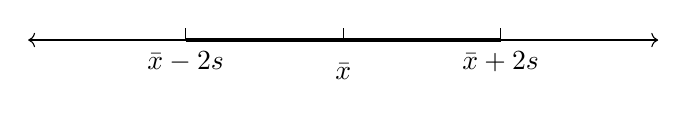
\begin{tikzpicture}
      % Draw main number line with arrows
      \draw[<->] (-4,0) -- (4,0);
      % Mark center point (x̄)
      \draw (0,0) node[below=5pt] {$\bar{x}$} -- (0,0.15);
      % Range markers
      \draw (-2,0) -- (-2,0.15) node[below=5pt] {$\bar{x} - 2s$};
      \draw ( 2,0) -- ( 2,0.15) node[below=5pt] {$\bar{x} + 2s$};
      % Range between -2s and +2s
      \draw[ultra thick, black] (-2,0) -- (2,0);    
    \end{tikzpicture}
    \end{center}
% --- Number Line --- 
        \item Outlier: a value far from the rest of the data
        \item[] \textit{Note: $x$ is an outlier if and only if $x < q_1 - 1.5(IQR)$ or $x > q_3 - 1.5(IQR)$}. Also, $1.5(IQR)$ tends to be known as a "mild" outlier where $3(IQR)$ tends to be known as an "extreme" outlier.
    \end{itemize}
    
    \noindent \textbf{Shape}
    \begin{itemize}
        \item Distribution: the "skyline" of a graph

% --- Shapes Examples ---
\begin{center}
\begin{tabular}{c c c}
% --- Row 1 ---
\begin{minipage}{0.3\linewidth}\centering
\begin{tikzpicture}[scale=0.45]
\begin{axis}[width=4cm, height=3cm, axis lines=left, xtick=\empty, ytick=\empty]
\addplot[domain=0:10, samples=2, thick] {0.5};
\end{axis}
\end{tikzpicture}\\
Uniform
\end{minipage}
&
\begin{minipage}{0.3\linewidth}\centering
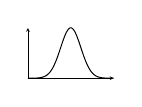
\begin{tikzpicture}[scale=0.45]
\begin{axis}[width=4cm, height=3cm, axis lines=left, xtick=\empty, ytick=\empty]
\addplot[domain=-3:3, samples=50, thick] {exp(-x^2)};
\end{axis}
\end{tikzpicture}\\
Bell-shaped
\end{minipage}
&
\begin{minipage}{0.3\linewidth}\centering
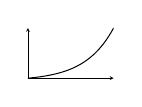
\begin{tikzpicture}[scale=0.45]
\begin{axis}[width=4cm, height=3cm, axis lines=left, xtick=\empty, ytick=\empty]
\addplot[domain=0:3, samples=50, thick] {exp(x)};
\end{axis}
\end{tikzpicture}\\
J-shaped
\end{minipage}
\\[1em]

% --- Row 2 ---
\begin{minipage}{0.3\linewidth}\centering
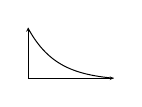
\begin{tikzpicture}[scale=0.45]
\begin{axis}[width=4cm, height=3cm, axis lines=left, xtick=\empty, ytick=\empty]
\addplot[domain=0:3, samples=50, thick] {exp(-x)};
\end{axis}
\end{tikzpicture}\\
Reverse J-shaped
\end{minipage}
&
\begin{minipage}{0.3\linewidth}\centering
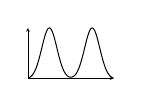
\begin{tikzpicture}[scale=0.45]
\begin{axis}[width=4cm, height=3cm, axis lines=left, xtick=\empty, ytick=\empty]
\addplot[domain=-4:4, samples=100, thick] {exp(-(x+2)^2) + exp(-(x-2)^2)};
\end{axis}
\end{tikzpicture}\\
Bimodal
\end{minipage}
&
\begin{minipage}{0.3\linewidth}\centering
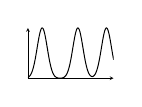
\begin{tikzpicture}[scale=0.45]
\begin{axis}[width=4cm, height=3cm, axis lines=left, xtick=\empty, ytick=\empty]
\addplot[domain=-6:6, samples=200, thick] {exp(-(x+4)^2) + exp(-(x-1)^2) + exp(-(x-5)^2)};
\end{axis}
\end{tikzpicture}\\
Multimodal
\end{minipage}
\end{tabular}
\end{center}
% --- Shapes Examples ---

        \item Skewness:
        \begin{itemize}
            \item if $\bar{x} > \tilde{x}$, then \textbf{right} or \textbf{positively skewed}
            \item if $\bar{x} < \tilde{x}$, then \textbf{left} or \textbf{negatively skewed}
            \item if $\bar{x} \approx \tilde{x}$, then \textbf{symmetrical}
            \item[] \textit{Note: These are not mathematical definitions of what skew means} 
        \end{itemize}
    \end{itemize}  



    \noindent \textbf{Other}
    \begin{itemize}
        \item Size (\(n\), \(N\))
        \begin{itemize}
            \item Also: $n_1, n_2, n_3$ or \(n\) and \(m\), etc.
            \item Given a data set consisting of \(n\) observations on some variable \(x\), the individual observations will be denoted by $x_1, x_2, x_3, ..., x_n$
       \end{itemize}    
    \end{itemize}  

% ---------------- Probability ------------------------------
\section{Probability}

% --- Set Theory ---
\subsection{Set Theory $\longrightarrow$ Probability Theory}
\begin{description}
    \item[Probability theory uses the foundations of set theory] 
\end{description}

\begin{center}
    \begin{tabular}{c|c}
        Set Theory & Probability Theory \\
        \hline
        universal set & sample set \\
        subset & event \\
        element & outcome \\
        disjoint & mutually exclusive \\
    \end{tabular}
\end{center}

    \begin{itemize}
        \item A set of all possible outcomes of an experiment is called a \textit{sample space}, noted by $\mathcal{S}$
        \item A subset of the sample space is called an $event$, noted by, for example:
        \begin{itemize}
            \item \{$A$, $B$, $C$, $D$,\ldots, $M$\} (beginning of alphabet; "reserved" letters are not used)
            \item \{$A_1$, $A_2$, $A_3$,\ldots\}
        \end{itemize}  
        \item[] An $event$ can be classified as:
        \begin{itemize}
            \item Simple: it consists of exactly one outcome
            \item Compound: it consists of more than one outcome
        \end{itemize}
        \item The \textit{empty set} is noted as $\emptyset =$ \{ \} 
        \begin{itemize}
            \item[] \textit{This is a \textbf{null event}: an event consisting of no outcomes whatsoever}
            \item[] Also called an \textit{impossible event}; this is only one example of an impossible event
            \item[] \textit{When $A \cap B = \emptyset$, $A$ and $B$ are said to be \textbf{mutually exclusive} or \textbf{disjoint}}
        \end{itemize}
        \item Elements of sample spaces are called $outcomes$
    \end{itemize}

\begin{description}
    \item[Example:] 3-coin flip (penny, nickel, then dime)
\end{description}

\begin{center}
\begin{tabular}{c c}
% --- Tree diagram (left) ---
\begin{minipage}{0.55\linewidth}
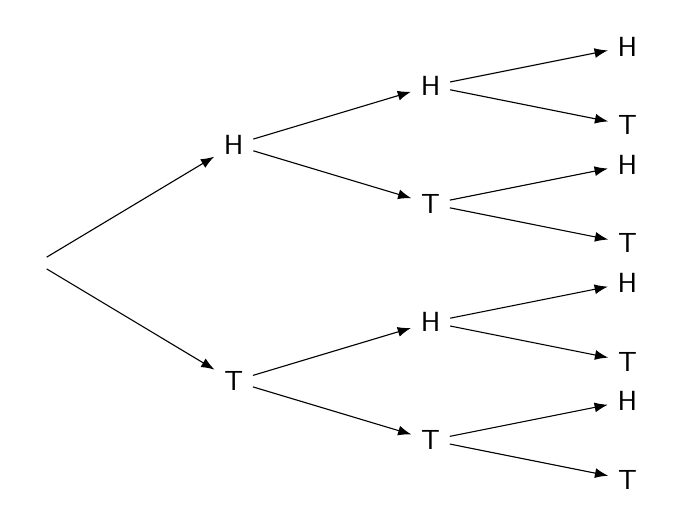
\begin{tikzpicture}[
  grow=right,
  level distance=25mm,
  edge from parent/.style={draw,-Latex},
  every node/.style={font=\sffamily}
]

\node {}
  child[sibling distance=30mm] { node {T}
    child[sibling distance=15mm] { node {T}
      child[sibling distance=10mm] { node {T} }
      child[sibling distance=10mm] { node {H} }
    }
    child[sibling distance=15mm] { node {H}
      child[sibling distance=10mm] { node {T} }
      child[sibling distance=10mm] { node {H} }
    }
  }
  child[sibling distance=30mm] { node {H}
    child[sibling distance=15mm] { node {T}
      child[sibling distance=10mm] { node {T} }
      child[sibling distance=10mm] { node {H} }
    }
    child[sibling distance=15mm] { node {H}
      child[sibling distance=10mm] { node {T} }
      child[sibling distance=10mm] { node {H} }
    }
  };
\end{tikzpicture}
\end{minipage}
&
% --- Table (right) ---
\begin{minipage}{0.35\linewidth}
\begin{tabular}{c c}
\hline
Outcome & \# Heads \\
\hline
HHH & 3 \\
HHT & 2 \\
HTH & 2 \\
HTT & 1 \\
THH & 2 \\
THT & 1 \\
TTH & 1 \\
TTT & 0 \\
\hline
\end{tabular}
\end{minipage}
\end{tabular}
\end{center}

\begin{itemize}
    \item $\mathcal{S}$ = \{HHH, HHT, HTH, HTT, THH, THT, TTH, TTT\}
    \item 1 and 2 heads most likely (3/8 each); 0 and 3 heads are least likely (1/8 each)
    \item Total events = $2^8 = 256$
    \begin{itemize}
        \item the number of possible events is the number of subsets of $\mathcal{S}$, always including at least the sample space and the empty set, e.g., $2^\mathcal{|S|}$ 
    \end{itemize}
    \item Possible events include:
    \begin{itemize}
        \item $A$: "All three coins show the same face" $\mathcal{S}$ = \{HHH, TTT\}
        \item $B$: "Has exactly two heads" $\mathcal{S}$ = \{HHT, HTH, THH\}
        \item $C$: "Has exactly one heads and two tails" $\mathcal{S}$ = \{TTH, THT, HTT\}
        \item $D$: "At least one tails appears" $\mathcal{S}$ = \{TTT, HHT, HTH, THH, TTH, THT, HTT\}
    \end{itemize}
    \item[] \textit{Note: Events $B$ \& $C$ are included in $D$; $A$, $B$, \& $C$ are mutually exclusive} 
\end{itemize}

% --- Relations ---
\subsection{Relations}

\begin{description}
    \item[The abstraction of $E$ and $F$:] 
\end{description}
\begin{itemize}
    \item $E \cap F$ = "elements of $\mathcal{S}$ that are contained in \textbf{both} $E$ and $F$" 
    \begin{itemize}
        \item [] \textit{The \textbf{intersection} of two events $A$ and $B$, read as "A and B," is the event consisting of all the outcomes that are in \textbf{both} A and B}
    \end{itemize}
    \item $E \cup F$ = "elements of $\mathcal{S}$ that are contained in \textbf{either} $E$ \textbf{or} $F$"
    \begin{itemize}
        \item [] \textit{The \textbf{union} of two events $A$ and $B$, read as "A or B," is the event consisting of all the outcomes that are in \textbf{either} A or B \textbf{or in both events} — that is, all outcomes in at least one of the events}
    \end{itemize}
    \item[] \textit{Note: $\cup$ = "intersect" and $\cap$ = "union"}
\end{itemize}

\begin{description}
    \item[The \textit{complement} of $E$, noted $E'$:] 
\end{description}
\begin{itemize}
    \item $E'$ = "element(s) of $\mathcal{S}$ that are \textbf{not} in $E$"
    \item[] \textit{The \textbf{complement} of an event $A$, denoted by $A'$, is the set of all outcomes that are not contained in $A$}
\end{itemize}

\begin{description}
    \item[De Morgan's Laws:] 
\end{description}
 \[ (A \cup B)' = (A') \cap (B') \]
 \[ (A \cap B)' = (A') \cup (B') \]

\begin{description}
    \item[Example:] 3-coin flip Continued
\end{description}
\begin{itemize}
    \item $A \cap B = \emptyset$
    \item $A \cap D =$ \{TTT\}
    \item $A \cup D = \mathcal{S}$
    \item $D' =$ \{HHH\}
    \item $A \cap B \cup D = D$ does not make sense, as indicating order is needed. Instead:
    \begin{itemize}
        \item $(A \cap B) \cup D = \emptyset \cup D = D$
        \item $A \cap (B \cup D) = A \cap D =$ \{$T$, $T$, $T$\}
    \end{itemize}
\end{itemize}

% --- Axioms, Interpretations, & Properties ---
\subsection{Axioms, Interpretations, \& Properties}

% ------------------ Counting ------------------------------
\section{Counting}

% --- {Product Rule} ---
\subsection{Product Rule}

% --- {Permutations & Combinations} ---
\subsection{Permutations \& Combinations}

% ------------------ Conditional Probability ------------------------------
\section{Conditional Probability}

% --- {Bayes' Theorem} ---
\subsection{Bayes' Theorem}

% --- {Independence} ---
\subsection{Independence}

% ------------------ Graphs & Visuals ------------------------------
\section{Graphs \& Visuals}

% --- Frequency & Relative Frequency Tables ---
\subsection{Frequency \& Relative Frequency Tables}

\textbf{Example:}
\begin{flushleft}
    \textit{Note: In-class data collection: favorite streaming services} \\
    \(n\) = 30 \\
    $\mathcal{S}$ = \{D, N, N, N, V,\ldots\}
\end{flushleft}

\begin{flushleft}
\begin{tabular}{c l c r r}
Value & Frequency & & & Relative Frequency \\ 
\hline
D & \tally{1} & = & 1 & $1/30 \approx 0.033$ \\
N & \tally{5} \tally{5} \tally{2} & = & 12 & $12/30 \approx 0.400$ \\
V & \tally{1} & = & 1 & $1/30 \approx 0.033$ \\
H & \tally{5} \tally{5} & = & 10 & $10/30 \approx 0.333$ \\ 
M & \tally{3} & = & 1 & $3/30 \approx 0.100$ \\
P & \tally{1} & = & 1 & $1/30 \approx 0.033$ \\
S & \tally{2} & = & 1 & $2/30 \approx 0.067$ \\
\hline
 & & & 30 & 1.000 \\
\end{tabular}
\end{flushleft}


% --- Histogram & Bar Graphs ---
\subsection{Histogram \& Bar Graphs}

\textbf{Qualitative Example:}
\begin{flushleft}
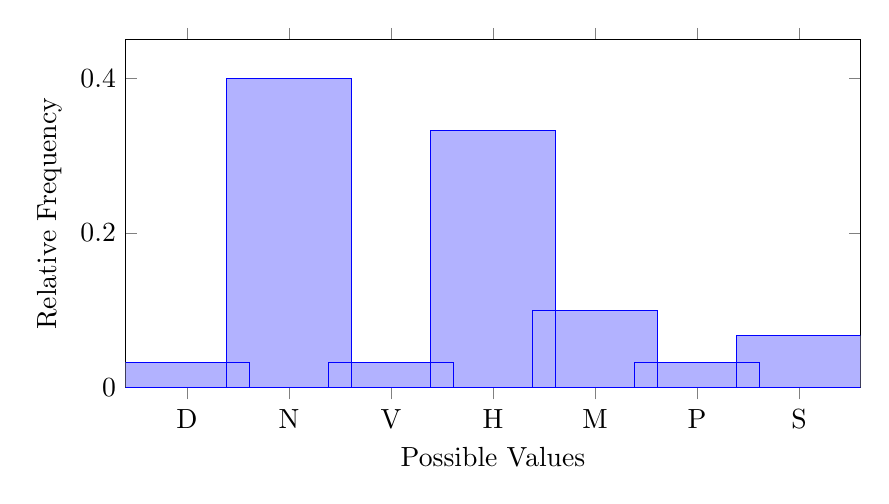
\begin{tikzpicture}
\begin{axis}[
    ybar,
    bar width=45pt,
    xlabel={Possible Values},
    ylabel={Relative Frequency},
    ymin=0, ymax=0.45,
    symbolic x coords={D,N,V,H,M,P,S},
    xtick=data,
    width=0.9\linewidth,
    height=6cm
]
\addplot coordinates {(D,0.033) (N,0.400) (V,0.033) (H,0.333) (M,0.100) (P,0.033) (S,0.067)};
\end{axis}
\end{tikzpicture}
\end{flushleft}
\textit{Note: Bars don't touch} \\

\noindent \textbf{Discrete Quantitative Example:}
\begin{flushleft}
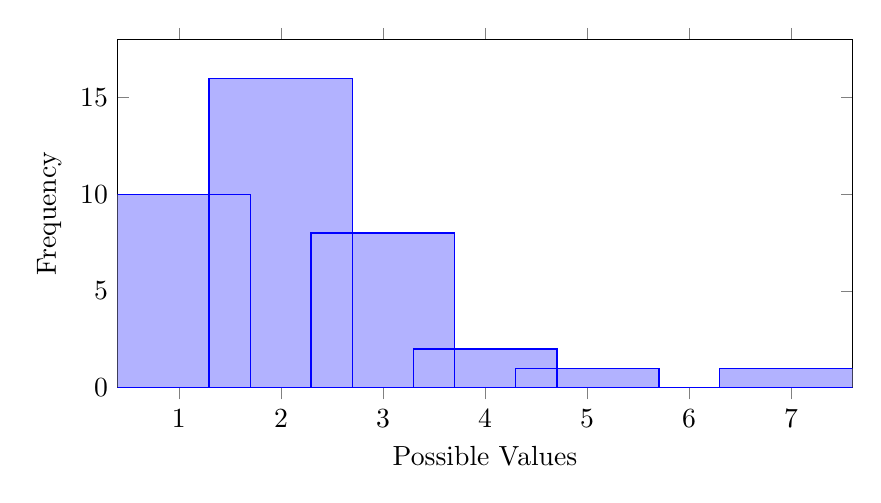
\begin{tikzpicture}
\begin{axis}[
    ybar,
    bar width=52pt,  
    xlabel={Possible Values},
    ylabel={Frequency},
    ymin=0, ymax=18,
    xtick=data,
    width=0.9\linewidth,
    height=6cm
]
\addplot coordinates {(1,10) (2,16) (3,8) (4,2) (5,1) (6,0) (7,1)};
\end{axis}
\end{tikzpicture} 
\end{flushleft}
\textit{Note: Bars touch; origin is not required to be zero} \\

\noindent \textbf{Continuous Quantitative Example:}
\begin{flushleft}
    \(n\) = 10 \\
    $\mathcal{S}$ = \{3.2, 3.5, 4.1, 16.8, 22.4, 25.7, 31.9, 36.3, 41.0, 44.6\}
\end{flushleft}

\begin{flushleft}
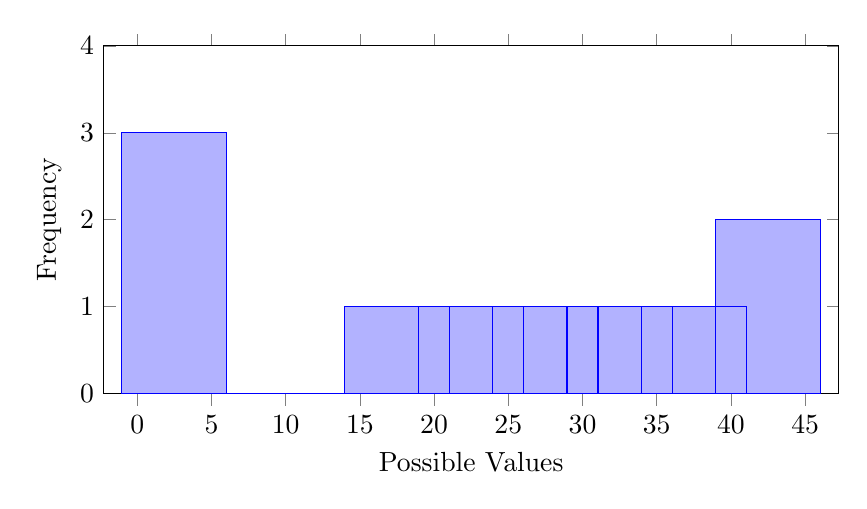
\begin{tikzpicture}
\begin{axis}[
    ybar,
    bar width=38pt,         
    xmin=0, xmax=45,
    ymin=0, ymax=4,
    xtick={0,5,...,45},
    xlabel={Possible Values},
    ylabel={Frequency},
    width=0.9\linewidth,
    height=6cm,
    enlarge x limits=0.05
]
\addplot coordinates {
    (2.5,3)  % midpoint of 0–5
    (7.5,0)  % 5–10
    (12.5,0) % 10–15
    (17.5,1) % 15–20
    (22.5,1) % 20–25
    (27.5,1) % 25–30
    (32.5,1) % 30–35
    (37.5,1) % 35–40
    (42.5,2) % 40–45
};
\end{axis}
\end{tikzpicture}
\end{flushleft}
\textit{Note: The x-axis must be subdivided into a suitable number of \textbf{class intervals} or \textbf{classes}, such that each observation is contained in exactly one class. Between 5–20 classes is satisfactory for most data sets, or\[\text{Number of classes} \;\approx\; \sqrt{\text{Number of observations}}\] The convention tends to be that an observation on a boundary is placed in the interval to the \textbf{right} of the boundary. The example provided here uses \textbf{equal-width} classes.} \\



% --- Stem-and-leaf Display ---
\subsection{Stem-and-leaf Display}
    \textbf{Construction:}
    \begin{enumerate} 
        \item Select one or more leading digit for the stem values
        \item[] \textit{Note: A display with 5–20 stems is recommended} 
        \item List \textbf{all possible} stem values in a vertical column 
        \item Record the leaf for each stem value \textbf{in ascending order} (unless created by hand) 
        \item Indicate the units for stems and leaves somewhere on the display 
    \end{enumerate}

    \begin{description}
        \item[Conveys:] typical/representative value, spread/distribution, gaps, symmetry, modes, outliers
        \item[] \textit{Note: Preserves the raw data to reconstruct as needed} 
    \end{description}

% --- Stem-and-leaf Display example ---
\begin{description}
\item[Example:] \{12, 13, 14, 14, 15, 21, 23, 25, 32\}

\begin{flushleft}
\begin{minipage}{0.55\linewidth}
\begin{tabular}{r|l}
1 & 2 3 4 4 5 \\
2 & 1 3 5 \\
3 & 2 \\
\end{tabular}
\end{minipage}%
\hfill
\begin{minipage}{0.4\linewidth}
\textit{Stem: Tens digit} \\
\textit{Leaf: Ones digit}
\end{minipage}
\end{flushleft}

\end{description}
% --- Stem-and-leaf Display example ---

% --- Dotplot ---
\subsection{Dotplot}
    \textbf{Construction:}
    \begin{enumerate} 
        \item Create horizontal measurement scale
        \item Place a dot above the corresponding location for each observation
        \item Stack observations vertically when they occur more than once
    \end{enumerate}

    \begin{description}
        \item[Conveys:] typical/representative value, spread/distribution, gaps, symmetry, modes, outliers
        \item[] \textit{Note: Emphasizes shape; can be crowded and imprecise when data sets are large} 
    \end{description}

% --- Dotplot example ---
\begin{description}
\item[Example:] \{2, 2, 3, 4, 4, 4, 5\}

\begin{flushleft}
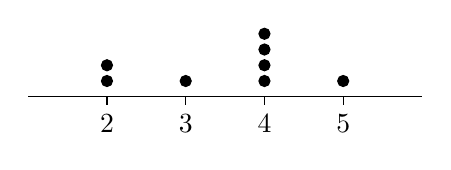
\begin{tikzpicture}[scale=1]
  % draw the axis
  \draw[-] (1,0) -- (6,0);
  \foreach \x in {2,...,5} {
    \draw (\x,0) -- (\x,-0.1) node[below] {\x};
  }

  % plot the dots
  \foreach \y in {0.2,0.4} \draw[fill] (2,\y) circle (2pt); % two 2's
  \foreach \y in {0.2}   \draw[fill] (3,\y) circle (2pt); % one 3
  \foreach \y in {0.2,0.4,0.6,0.8} \draw[fill] (4,\y) circle (2pt); % three 4's
  \foreach \y in {0.2}   \draw[fill] (5,\y) circle (2pt); % one 5
\end{tikzpicture}
\end{flushleft}

\end{description}
% --- Dotplot example ---

% --- Boxplot ---
\subsection{Boxplot}
    \textbf{Construction:}
    \begin{itemize}
        \item Left edge of the "box" is at the lower fourth/quartile; right edge at the upper fourth/quartile (so box width = $f_s$ or $IQR$)
        \item Vertical line segment inside the box at the median
        \item Draw whiskers to the largest and smallest observations (non-outliers)
        \item Mild outliers are indicated by closed circles; extreme outliers are indicated by open circles
        \item Comparative box plots can be constructed vertically or horizontally
        \item The LaTeX PGFplots package includes styling that is not always consistent with the standards included here (e.g., outlier indications, endcaps on whiskers, etc.)
    \end{itemize} 

    \begin{description}
        \item[Conveys:] describes several of a data set's most prominent features, e.g., center, spread, symmetry (or lack thereof), and outliers AND can compare multiple data sets against each other
        \item[] \textit{Note: "Resistant" to outliers} 
    \end{description}

% --- Boxplot Example ---

\begin{tikzpicture}
\begin{axis}[
    ytick={1,2,3},
    yticklabels={Group A, Group B, Group C},
    boxplot/variable width,
]
    \addplot+ [% Group A:
        boxplot prepared={
            lower whisker=42, lower quartile=45,
            median=47,
            upper quartile=47.5, upper whisker=48,
            sample size=1000,
        },
    ] table [row sep=\\,y index=0] { 40\\ 34\\ 56\\ };
 
    \addplot+ [% Group B:
        boxplot prepared={
            lower whisker=36, lower quartile=39,
            median=40,
            upper quartile=41, upper whisker=43,
            sample size=100000,
        },
    ] coordinates {};
 
    \addplot+ [% Group C:
        boxplot prepared={
            lower whisker=41, lower quartile=44,
            median=45,
            upper quartile=46, upper whisker=47,
            sample size=50000,
        },
    ] coordinates {(0,35) (0,55)};
\end{axis}
\end{tikzpicture}

\noindent 
\textit{Note: This example includes sample size scale styling} 


% --- Scatter Plot ---
\subsection{Scatter Plot}


\newpage
\nocite{*}
\printbibliography[title={References}]

\end{document}

